\section{Editor Design}
The editor is used by the player to design their program that will be run during the game. To keep the overall design experience, the editor will be using the same hexagonal design as the playing field. The programming will be done visually, and the hexagonal design will give the user more options for organizing their program.

The editor consists of two main parts, the programming grid of hexagons on the left, and individual fine tuning of elements on the right, an illustration can be seen on \autoref{fig:editor}.

\begin{figure}[h]
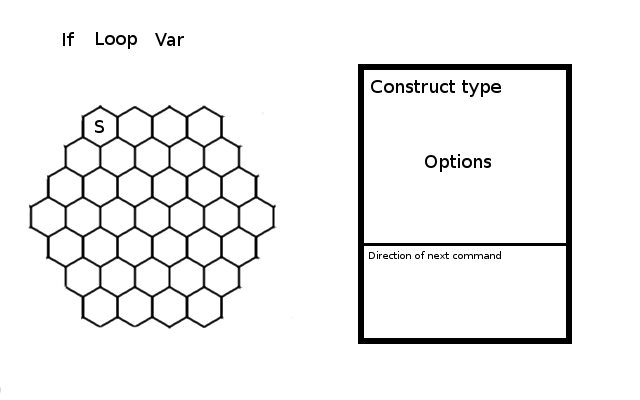
\includegraphics[width=\textwidth]{img/editor.png}
\caption{Preliminary design of the editor.}
\label{fig:editor}
\end{figure}

\subsubsection*{Programming Grid}
The programming grid makes use of a drag and drop interface, each programming construct such as if statements and loops, can be dragged from the top of the screen onto the hexagonal grid. This hexagonal grid only has a start point in the beginning of a game, and it is up to the player to create the program itself. The program will be running from the start point on the grid to a user defined end point, this end point is created by simply letting the program run outside the hexagonal grid. By doing this, the player is essentially creating a loop that the program will be running in during its execution.\newline

As the editor is using a drag and drop interface, it is very easy to add new functionality to a program, just drag a construct onto the path of the current program, and define variables if needed. As the aim of the game is to teach programming without doing so explicitly, the variables are divided into categories with three of each. These are numbers, entities, and directions. The idea is that by limiting variables to three easy to understand categories, the player will be able to understand what happens without prior knowledge to programming.

\subsubsection*{Details Pane}
Different constructs will have different options to specify this is where the details pane on the right of the hexagonal grid comes into play. The details pane is activated when the player clicks on a construct that has been placed on the hexagonal grid.\newline

The details pane will show different information depending on what kind of construct the player has clicked on. For example, an the options for an if will show a list of variables that the if can compare with to generate a scenario where the variable can be in a true or false state, making the if work. A move construct, however, will only show a direction it will move in. The bottom part of the details pane is used by the player to choose which tile on the hexagonal grid the program should be going to next. This is can be used to structure the program or make it possible for the player to customize the grid to their liking.

\subsection{Design Decisions}
Several decisions have been taken with the design of the editor, firstly it was clear from the beginning that the editor should utilize some kind of visual interface for programming. If the player had to write code explicitly it would be very clear that the game is trying to teach programming, and the goal of teaching without the player noticing would very quickly be impossible to achieve.\newline

When it was decided that the programming interface would be visual, the idea of a grid quickly became the preferred method. As described in section \todo{refer to Carnage Heart section}, the game Carnage Heart have previously made use of a similar grid interface for programming, it was chosen that the editor should keep the look and feel from the game board, and thus it also makes use of a hexagonal grid. The hexagonal grid has some features which made preferable to a standard square grid. The hexagonal grid makes it possible for the player to have more options as to how the program is structured, it also makes it possible for the two branches of an if statement or a loop to be next to each other rather than on different sides of a square.\newline

The details pane was more difficult to get right. When it was chosen that the editor should utilize a visual programming interface with drag and drop, the player would need to be able to set some amount of variables for the program to be functional enough. The details pane was chosen because it removes the need to exit out of the details pane to be able to switch to the details of another construct on the grid, if the details were to pop up over the hexagonal grid. The details pane on the side of the hexagonal grid effectively eliminates a number of steps which makes the game quicker and less frustrating to use.
